%===================================================================================
% Chapter: IDS
%===================================================================================
\chapter{Sistema de Detección de Intrusos}\label{chapter:ids}
% \addcontentsline{toc}{chapter}{Sistema de Detección de Intrusos}
%===================================================================================

Entre los años 1984 y 1986, Dorothy Denning y Peter Neumann desarrollaron un primer modelo de IDS \cite{denning1985requirements} para proteger los sistemas de cómputos. Pertenecen a la rama de la computación de las redes aunque en los últimos tiempos se han aplicado para su creación técnicas de distintas disciplinas como son algunas de inteligencia artificial. En la última década se han logrado avances en esta tecnología, obteniendo mejores resultados. A pesar de ello no se ha logrado un sistema con una efectividad lo suficientemente alta y aún es una línea de investigación activa. Se considera que estos sistemas tienen una gran importancia, ya sea económica o social, al proteger los datos delicados que viajan por la red y mantener la privacidad de cada usuario. Entre las técnicas de inteligencia artificial más utilizadas se encuentra el aprendizaje de máquinas.

\section{Tipos de sistemas}
Existen varios tipos de IDS, pero para el propósito de este documento se pueden separar en basados en la red y basados en el host. En el caso de los basados en la red monitorean el tráfico de ella, analizan su actividad y la de los protocolos de aplicaciones en búsqueda de actividad sospechosa. Usualmente se colocan en los límites entre redes, como próximos a los cortafuegos de borde, routers, servidores de red privada virtual (VPN por sus siglas en ingles), servidores de acceso remoto o dispositivos de redes inalámbricos, entre otros. Los basados en el host monitorean las características de un solo equipo y los eventos que ocurren dentro de él. Pueden monitorear la red del equipo donde se encuentra el software, los registros del sistema, procesos en ejecución, aplicaciones activas, acceso y modificación de ficheros además de aplicaciones del sistema que cambien la configuración. En su mayoría se implementan en equipos críticos como servidores con acceso público o con información delicada.

Cada una de estas clasificaciones puede ser separada a su vez en las siguientes:

\begin{itemize}
    \item \textbf{Detección basada en firmas:} una firma es un patrón que corresponde a una amenaza conocida. Este proceso compara firmas en eventos observados para identificar posibles incidentes. Es muy efectivo detectando patrones iguales a los que almacena pero tienen un gran número de fallos cuando se trata de amenazas no registradas, disfrazadas con el uso de técnicas de evasión o variaciones de las ya conocidas.
    \item \textbf{Detección basada en anomalías:} es el proceso de comparar definiciones sobre cual actividad es considerada normal en los eventos observados para identificar desviaciones significantes. Utiliza una serie de perfiles que representan el comportamiento normal de varios elementos como usuarios, hosts, conexiones de red o aplicaciones. Por ejemplo, el perfil para una red empresarial en una hora normal de trabajo muestra que en la navegación web se consume el 13\% del ancho de banda total. Si el sistema detecta una diferencia considerable en este parámetro podría significar que la red se encuentra bajo una amenaza. Los perfiles pueden ser configurados para varios comportamientos, como el número de correos electrónicos enviados por un usuario, la cantidad de intentos fallidos al iniciar sesión por un host o el tiempo de uso de un proceso determinado. Una de las ventajas de este método es que es muy efectivo ante amenazas desconocidas.
    \item \textbf{Análisis de protocolo con estados:} compara perfiles predeterminados de definiciones generalmente aceptadas de actividad no maliciosa por cada uno de los estados de protocolos contra eventos observados para identificar desviaciones. A diferencia de la detección basada en anomalías, que utiliza perfiles de host o de redes específicos, esta se basa en perfiles universales desarrollados por el proveedor que especifica cuales protocolos y cuales no deben ser usados. La parte de estados en el nombre del método quiere decir que el sistema es capaz de entender, darle seguimiento al estado, transportar y tener una noción de los protocolos de aplicaciones. Por ejemplo, cuando un usuario inicia una comunicación por el protocolo de transferencia de archivos (FTP por sus siglas en ingles), el estado inicial es de no autenticado. En esta fase los usuarios solo deberían poder ejecutar unos pocos comandos como una petición de ayuda o enviar nombre de usuario y contraseña. Una parte importante de entender el estado es emparejar pedidos con respuestas, para cuando ocurra un intento de autenticación FTP, se pueda determinar si fue satisfactorio encontrando el código de confirmación en el mensaje de respuesta correspondiente al pedido. En caso de que el usuario complete la autenticación entonces podrá utilizar los comandos disponibles. Por otra parte, si se intenta utilizar alguno de estos en un estado que no se le ha confirmado la autenticación, se puede considerar como actividad sospechosa. Los sistemas de análisis de protocolo con estados pueden identificar una secuencia de comandos no esperados, en caso de que se necesite un orden específico y recordar si una sesión está autenticada o no. El análisis de protocolo en el nombre significa que realiza un chequeo exhaustivo de las características de los comandos individuales, como puede ser la longitud mínima y máxima de los argumentos.
\end{itemize}

\section{Problemas fundamentales}
Los IDS basados en técnicas de aprendizaje de máquinas son sistemas entrenados con un determinado conjunto de datos que son empleados más adelante en la detección de intrusos a una red. Una revisión general al proceso de filtrado de paquetes permite identificar los siguientes problemas:
\begin{itemize}
    \item Detección de comportamiento no observado.
    \item Porcentaje de detección de intrusos.
    \item Falsos positivos.
    \item Falsos negativos.
    \item Equipo final para su implementación.
    \item Tipo del ataque.
\end{itemize}

Esta investigación se centra en los problemas de los casos no observados, falsos positivos y falsos negativos, aplicados sobre el conjunto de datos NSL-KDD, determinando si un paquete de red posee un comportamiento normal o anómalo. A pesar de que en \cite{goyal2008ga,ahmadi2009intrusion} trabajan con el conjunto de datos KDD99, atacan el problema de clasificación con dos variantes diferentes de algoritmos genéticos. En otra investigación \cite{samrin2018hybrid} proponen el uso del algoritmo k-medias para el agrupamiento en subconjuntos donde cada uno contenga datos de un solo tipo de ataque, crear y entrenar $n$ redes neuronales(una por cada tipo de ataque diferente) y con esto crear un método de conjunto(\textit{Ensemble learning}). 

El trabajo \cite{almseidin2017evaluation} ofrece una comparación de varios algoritmos, mostrando el de árboles aleatorios mejores resultados que el resto. Esta mejora se puede apreciar en \cite{anani2018recurrent}, que se busca minimizar el tiempo de entrenamiento de redes neuronales recurrentes sobre KDD99, utilizan dos algoritmos para la reducción de dimensiones de los datos y árboles aleatorios vuelve a mostrar mejores resultados. Utilizando ese mismo conjunto de datos se tiene \cite{kabanda2019bayesian}, aquí realizan un análisis de varios algoritmos y de las características de los datos. Como propuesta de reducción de dimensiones se tiene \cite{sammany2007artificial,divyasree2018network}, en el primer caso no se especifica como se realizó y en el segundo caso solo trabajan con las características básicas y de contenido, ignorando las de tráfico; para la clasificación de cada ataque por separado seleccionan 10 de las características que utilizan con el algoritmo de \textit{chi cuadrado}

Este trabajo se realizó sobre el conjunto de datos NSL-KDD, que es una mejora del conjunto original KDDCup99. De igual manera se puede encontrar el trabajo \cite{abualkibash2019machine}, en el presentan resultados de varios algoritmos diferentes, nuevamente mostrando buenos resultados con árboles aleatorios. En este caso utilizan el conjunto de prueba que se encuentra en NSL-KDD. Por otra parte, en \cite{ludwig2019applying} no se especifican si los resultados fueron obtenidos utilizando dichos datos de prueba, su forma de enfrentar el problema es con métodos de conjunto utilizando varias redes neuronales. De las bibliografías consultadas, la única que ofrece una observación sobre la predicción de los datos que no estuvieron presentes en la fase de entrenamiento del algoritmo es \cite{abualkibash2019machine}.

\section{Fases de la detección y prevención de intrusos}
Los problemas tratados en esta tesis pueden ser enmarcados como sistemas de detección de intrusos, estos forman parte de los sistemas de detección y prevención de intrusos, los que están compuestos por las siguientes fases:

\begin{itemize}
    \sloppy
    \item Almacenar información relacionada con los eventos observados. Usualmente la información es almacenada de forma local y puede ser enviada a otros sistemas como un servidor central encargado de archivar todos los eventos, información de seguridad, administradores de solución de eventos y sistemas de administración empresarial.
    \item Notificar a los encargados de la seguridad de un evento de importancia observado. Esta notificación, conocida como alerta, es enviada por cualquier vía de mensajes ya sea un correo electrónico, una página web o programas definidos por el usuario. La notificación normalmente incluye la información básica del evento. El administrador debe acceder al sistema para una mayor especificación.
    \item Elaborar un reporte. Los reportes resumen los eventos monitoreados y facilitan detalles sobre algún evento en particular de interés.
\end{itemize}

Los sistemas de prevención de intrusos se diferencian de los sistemas de detección de intrusos por una característica: los sistemas de prevención pueden responder en caso de la detección de una amenaza y prevenir que esta ocurra satisfactoriamente.

\section{Redes neuronales}

Las redes neuronales artificiales (RNA o ANN por sus siglas en inglés) son algoritmos de la rama de la inteligencia artificial que dado un conjunto de datos de ejemplo, ofrecen una función, sin importar el dominio de los valores de entrada y de salida, capaz de aproximar el resultado. Han brindado resultados excelentes en el reconocimiento de escritura a mano, palabras en audios y rostros.

Los primeros acercamientos a esta nueva tecnología fueron a principios de los a\~nos 1950 inspirados en los sistemas de aprendizaje biológicos. Son un conjunto de unidades simples, conectadas de manera densa entre ellas, donde cada unidad toma un real (que puede ser o no la salida de otra) y produce como resultado otro valor real (que puede convertirse en la entrada de otra unidad). El cerebro humano se estima que posee una red neuronal con $10^{11}$ unidades densamente conectadas, cada una de ellas conectadas con otras $10^{4}$ en promedio. La velocidad de comunicación entre una neurona y otra se encuentra en el orden de $10^{-3}$ segundos, por otra parte, las computadoras poseen una velocidad de $10^{-10}$ segundos. Los humanos son capaces de tomar complejas decisiones sorprendentemente rápido. Un ejemplo de esto es el reconocimiento de rostros, a un humano promedio le toma aproximadamente $10^{-1}$ segundo reconocer visualmente a su madre. Teniendo en cuenta la velocidad de comunicación entre neuronas, este proceso no excede unos cientos de pasos. Esto ha llevado a la comunidad científica a pensar que el sistema neuronal biológico es capaz de realizar tareas de procesamiento de información de manera altamente paralelas distribuidas en varias neuronas. Una de las motivaciones principales es lograr un sistema capaz de hacer procesos altamente paralelos en representaciones distribuidas \cite{brown1990learning,churchland1992computational,mitchell1997machine}.

Después de los primeros pasos en la creación de las redes neuronales, los científicos se encontraron con el problema de entrenar grandes arquitecturas de una forma eficiente. A mediados de los a\~nos 1980, varios estudios de diferentes partes del mundo, descubrieron de forma independiente el algoritmo de propagación hacia atrás, el cual utiliza el método de optimizaci\'on de descenso por gradiente para entrenar cadenas de operaciones param\'etricas. Unos de los pioneros en utilizar estas técnicas con grandes éxitos fueron los laboratorios Bell, cuando Yann LeCun utilizó las ideas iniciales de las redes convolucionales y la propagación hacia atrás. Como resultado obtuvieron una red que podía reconocer dígitos escritos a mano con alta efectividad, la cual nombraron LeNet \cite{lecun1995comparison}, y fue utilizada por el Servicio Postal de los Estados Unidos en la década de 1990. A pesar de que las redes neuronales artificiales fueron inspiradas por el sistema biológico, ambas poseen características que las diferencian.

\subsection{Estructura}
Las redes neuronales artificiales reciben este nombre por su composición. Están conformadas por varias neuronas interconectadas entre s\'i como se puede observar en la figura \ref{fig:neural_network}. Existen varias formas de conexión pero una de las más populares es la densa donde cada neurona se encuentra completamente conectada a todas las de la capa anterior y posterior. Estas conexiones se les conoce como pesos y en el proceso de entrenamiento se van modificando hasta obtener el resultado deseado. Todas las redes constan de tres capas:

\begin{itemize}
    \item \textbf{Capa de entrada:} usualmente posee tantas neuronas como características tengan los datos.
    \item \textbf{Capas ocultas:} puede ser una sola o varias capas, el numero puede variar en dependencia de la complejidad del modelo. Envían los datos a través de la sinapsis desde la capa de entrada hasta la de salida.
    \item \textbf{Capa de salida:} última capa de cualquier modelo. Es la que ofrece los valores resultantes de los cálculos.
\end{itemize}

\begin{figure}[h]
    \centering
    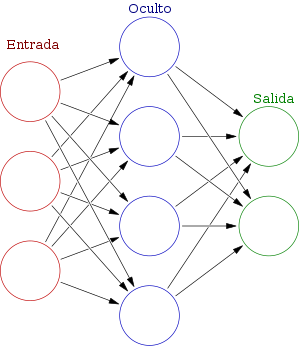
\includegraphics[width=.6\linewidth]{Images/neural_network.png}
    \caption{Estructura básica de una red neuronal.}
    \label{fig:neural_network}
\end{figure}

Cada capa puede poseer una o más neuronas, matemáticamente, estas se definen por $f(x) = k(\sum_{i}w_{i}g_{i}(x))$, donde $k$ es la función de activación, $w$ es el vector de los pesos asociados a cada conexión y $g(x)$ son los valores resultantes de la capa anterior. Las funciones de activación en la mayoría de los casos se utilizan algunas ya definidas como pueden ser la tangente hiperbólica, la función sigmoide o la unidad lineal rectificada (ReLU, por sus siglas en inglés), entre otras. En este trabajo se utilizó la función sigmoide para la capa de salida: \[f(x) = \frac{1}{1 + e^{-x}}\] y ReLU para las capas intermedias: \[f(x)=max(0,x)\]
Esto se debe a que la simplicidad de ReLU permite agilizar el proceso de entrenamiento y cuando existen muchas capas, la función sigmoide, puede hacer que las neuronas desaparezcan dado que sus valores tienden a 0. La parte final de todo modelo es la función de pérdida y un optimizador; la primera es la encargada de comparar las predicciones con el valor real de los datos, ofreciendo un valor de pérdida, mientras que el optimizador es el encargado de recibir estos valores para reajustar los pesos. Como el problema que se está enfrentando en este trabajo es de clasificación binaria y la salida de la red es una probabilidad es mejor utilizar $binary_crossentropy$ como función de pérdida. Existen otras opciones pero esta es la más utilizada en los modelos que la salida es un valor de probabilidad \cite{10.5555/3203489}.
% TODO: justificar la eleccion del optimizador

Existen dos tipos de redes principales. La que se muestra en la figura \ref{fig:neural_network} se le conoce como alimentación hacia adelante, dado que su estructura es un gráfico dirigido acíclico. Las redes con ciclos reciben el nombre de recurrentes. En ellas la función de las neuronas tiene una dependencia sobre s\'i misma que puede estar basada en el tiempo. Este trabajo se centra en explorar los resultados del primer tipo mencionado en la detección de intrusos por lo que todos los modelos utilizados tienen estructuras ac\'iclicas.

En el proceso de entrenamiento de una red neuronal usualmente se itera sobre los datos varias veces (\textit{epochs}) para obtener una mejor generalización (tener buenos resultados cuando se enfrenta a entradas que no ha visto). Esto le da la oportunidad a la red de ver los datos anteriores y reajustar sus parámetros para que el modelo no esté sesgado hacia los últimos que procesó durante el entrenamiento. Esta tarea se realiza en pequeños lotes o \textit{batch} que no es más que un subconjunto de los datos.

Un problema común entre los algoritmos de aprendizaje de máquina es el sobreajuste. Esto se puede presenciar cuando el comportamiento del modelo ante los datos de validación alcanza su punto máximo y luego comienza degradarse. Existen varias formas de lidiar con el sobreajuste aunque el \textit{dropout} es una de las más efectivas. Solo se ejecuta en el proceso de entrenamiento y se aplica a las capas de la red. Consiste en la desactivaci\'on aleatoria de algunas de las características de salida de la capa en la que se encuentra, por ejemplo, si el factor de desactivaci\'on es de $0.5$ y la salida toma los valores [1, 0.7, 2.1,  0.3], se desactivan la mitad de las características y el resultado podría ser [1, 0, 0, 0.3].
% TODO: explicar el backpropagation

\subsection{Aplicaciones}
Las redes neuronales artificiales pueden utilizarse para resolver diversos problemas. En la práctica los resultados obtenidos han sido muy buenos. Por lo general se aplican en escenarios donde la entrada puede representada por varios pares de atributos, la salida de la función objetivo puede ser de cualquier tipo, los ejemplos de entrenamiento pueden contener errores, se requieren de largos tiempos de entrenamiento, se requiere de una rápida evaluación de los datos, no es necesario que los humanos comprendan la función objetivo aprendida, entre otras características.

A lo largo de la historia se han utilizado para la solución de disímiles problemas. De forma general, las áreas en las que se aplican son la predicción de funciones \cite{naccha2012prediction}, clasificación \cite{lecun1995comparison}, procesamiento de datos \cite{montano2017redes}, robótica \cite{madrigal2002robots} e ingeniería de control \cite{forero2013control}. La detección de intrusos se puede definir como un problema de clasificación dado que después de analizar los datos se debe decidir si estos son tráfico normal o anómalo, en algunos casos también se especifica el tipo de ataque.

\section{Conjunto de datos y características}
Distintas investigaciones se han enfocado en realizar sistemas de detección de intrusos teniendo como fuente de datos NSL-KDD. En 1998 la Agencia de Proyectos de Investigación Avanzados de Defensa, más conocida por su acrónimo DARPA, recopiló y almacenó la información del tráfico de una red que nombró KDDCup99 llegando a ser uno de los conjuntos de datos públicos que contiene diferentes ataques vigentes en la actualidad y más utilizados por la comunidad científica. NSL-KDD fue diseñado para resolver varios de los problemas existentes en el conjunto original como son la información redundante, tanto en los conjuntos de entrenamiento como de prueba, y la cantidad de datos en cada subconjunto es razonable, lo cual hace comparable y consistentes los resultados de cualquier trabajo y evita tener que escoger un subconjunto aleatorio para los diferentes procesos.

\subsection{Propuesta de Proceso de Detección de Intrusos en el conjunto de datos}
Determinar si un paquete es malicioso, es una problemática que involucra diferentes procesos y alternativas de solución. Encontrar una combinación de algoritmos que se ajuste a las características particulares de este problema, permitiría establecer una propuesta general.

La solución que se propone para el proceso de detección de intrusos en NSK-KDD se divide en 3 etapas:

\begin{itemize}
    \item Procesamiento y normalización de los datos
    \item Reducción de dimensiones o eliminación de características no relevantes.
    \item Clasificación.
\end{itemize}

En cada etapa pueden ser utilizados diferentes algoritmos dependiendo de las características del problema a resolver en cada una de ellas. Para esto es necesario identificar que algoritmos son los más prometedores así como la mejor combinación de ellos.

\subsection{Bosques aleatorios}
Para el proceso de reducción de dimensiones en los datos se utilizó el algoritmo de bosques aleatorios \cite{breiman2001random}. Después de la revisión de varios artículos \cite{almseidin2017evaluation,anani2018recurrent, abualkibash2019machine, hasan2016feature} este mostró buenos resultados para el problema en cuestión, en algunos casos como clasificador y en otros para la selección de las características con mayor relevancia en los datos. Es un algoritmo que ofrece un buen rendimiento en muchos problemas y por su facilidad a la hora de entrenar y ajustar ha ganado gran popularidad.

En su estructura, está compuesto por $N$ de árboles de decisión. Para el árbol $k$ se genera un vector aleatorio con una muestra de los datos de entrenamiento, este es independiente a los $k - 1$ generados anteriormente aunque poseen la misma distribución; el árbol es entrenado con su respectivo vector dando como resultado un clasificador. Luego de este proceso, para un dato $x$, se escoge la clase que mayor cantidad de árboles haya clasificado.

La unidad básica de este algoritmo son los árboles de decision y como su nombre lo indica poseen una estructura de árbol. Estos se utilizan en los problemas donde la función objetivo tiene como salida valores discretos. Por su funcionamiento se pueden representar como un conjunto de condiciones ($if/then$). Cada nodo de un árbol representa una prueba a una característica de los datos y este posee tantas ramas como valores diferentes tome esta. La cuestión principal de este algoritmo es la decisión de cual característica se prueba en cada nodo.

De forma simplificada, su funcionamiento se puede observar en la tabla siguiente, este ofrece resultados \textit{booleanos}.

\begin{verbatim}
    AD(Ejemplos, Característica_objetivo, Características)
        Ejemplos es el conjunto de datos de entrenamiento.
        Característica_objetivo es la característica que tiene
        los valores que el árbol debe predecir.
        Características es la lista del resto de las
        Características de los datos que el árbol debe probar.
        Devuelve como resultado un árbol que clasifica
        correctamente los Ejemplos.

    - Crear el nodo raíz del árbol.
    - Si todos los ejemplos son positivos, devolver la raíz
    con la etiqueta positiva.
    - Si todos los ejemplos son negativos, devolver la raíz
    con la etiqueta negativa.
    - Si las características están vacías, devolver la raíz
    con la etiqueta del valor más común de
    Característica_objetivo en Ejemplos.
    - En otro caso:
        - A <- la característica que mejor clasifique los
        Ejemplos.
        - Asignar la característica A a la raíz.
        - Por cada posible valor v de A:
            - Añadir una nueva rama a la raíz para cuando
            A tome el valor v.
            - E' <- subconjunto de los Ejemplos que toman
            el valor v en la característica A.
            - Si E' esta vacío:
                - Entonces añadir un nodo hoja a esta rama
                con la etiqueta del valor más común de
                Característica_objetivo en Ejemplos.
            - En otro caso añadir el sub-árbol resultante de
                AD(Ejemplos, 
                   Característica_objetivo, 
                   Características - {A})
\end{verbatim}

Para poder definir cual es la mejor característica que clasifica los ejemplos se utiliza la ganancia de información. Si se tiene un conjunto $S$ de ejemplos, la ganancia de información para la característica $A$ se puede definir como:
\[GI(S, A) \equiv E(S) - \sum_{v \in Values(A)} \frac{|S_{v}|}{|S|}E(S_{v})\]
donde $Values(A)$ son todos los posibles valores que puede tomar la característica $A$, $S_{v}$ es el subconjunto de $S$ donde la característica $A$ toma el valor $v$ y la función $E$ es la entropía de un conjunto. Si los valores objetivos que el árbol debe predecir toman $c$ clases diferentes y $p_{i}$ es la proporción de $S$ que pertenece a la clase $i$, entonces la entropía se define como:
\[E(S) \equiv \sum_{i=1}^c -p_{i}log_{2}(p_{i})\]

Como se ha mostrado, la base de este algoritmo es la selección de las  características más importantes. Como se mencionó anteriormente, bosques aleatorios es la unión de varios árboles de decisión, cada uno entrenado con una porción aleatoria de los datos. Esto permite que la elección de la importancia de cada característica varíe en cada árbol. Los bosques aleatorios promedian la importancia brindada por cada árbol ofreciendo un mejor resultado general.